\subsubsection{Use Case}
			\paragraph{Registration of a new taxi driver}
			\begin{center}
			~\\
			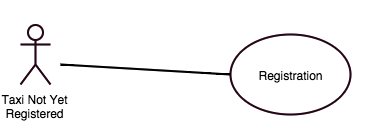
\includegraphics[width=0.60\textwidth]{./images/UseCaseTaxiNotYetRegistered.png}~
			\end{center}
			\begin{tabular}{l l}
		 \textbf {Name} & Registration  \\ \hline
		 \textbf{Actors} & Taxi not yet registered \\ \hline
		 \textbf{Entry conditions} & No entry conditions \\ \hline
		 \textbf{Event flow} & 
		 \parbox{0.7\textwidth}{
		 \begin{enumerate}
		 \item The new taxi driver not yet registered
		    \begin{itemize}
		    \item opens the myTaxiService mobile application;
		    \item clicks on "Sign In" link;
		    \item inserts name, surname, email address and a password for the login, after the opening of a new window;
		    \item clicks on "Confirm" link;
		    \end{itemize}
		 \item the system assigns an identifier, that is the taxi plate of the new taxi and which will be used by the new taxi driver as his username for the login.
		 \end{enumerate}
		 } \\ \hline
		 \textbf{Exit Condition} &  \parbox{0.7\textwidth}{The system adds the new taxi driver in the database and it grants him access to the application.} \\ \hline
		 \textbf{Exceptions} & Password inserted wrongly.
		\end{tabular}
		
		\newpage
		\paragraph{User side}
			\begin{center}
			~\\
		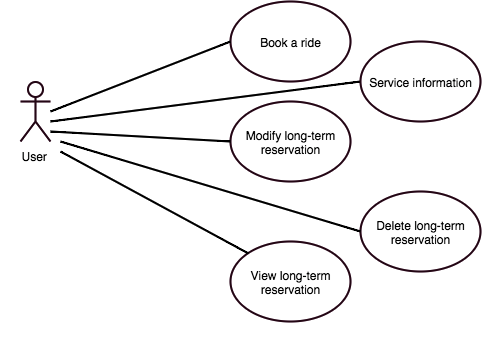
\includegraphics[width=0.90\textwidth]{./images/UseCaseUser.png}~
			\end{center}
		\newpage
		\subparagraph{Booking a ride}
		~\\[0.2cm]
			\vspace{20pt}
		\noindent
		
		\begin{tabular}{l l}
		 \textbf {Name} & Book a short-term reservation  \\ \hline
		 \textbf{Actors} & User, Taxi \\ \hline
		 \textbf{Entry conditions} & No entry conditions \\ \hline
		 \textbf{Event flow} & 
		 \parbox{0.7\textwidth}{
		 \begin{enumerate}
		 \item The user accesses to the web site or the mobile application.
		 \item The user clicks on "Book a ride".
		 \item The user inserts name, surname, phone number and address.
		 \item The user clicks on the "Confirm" button.
		 \item The system inserts the data of the user in the database.
		 \item The system identifies the area in which the address specified by the user is.
		 \item The system selects the first available taxi from the taxis queue.
		 \item The system sends the notification to the taxi.
		 \item The system sends a confirmation via SMS to the user.
		 \end{enumerate}
		 } \\ \hline
		 \textbf{Exit Condition} & \parbox{0.7\textwidth}{ The system adds the user information in the database.}\\ \hline
		 \textbf{Exceptions} & Address inserted wrongly.
		\end{tabular}
		
		\begin{tabular}{l l}
		 \textbf {Name} & Book a long-term reservation  \\ \hline
		 \textbf{Actors} & User, Taxi \\ \hline
		 \textbf{Entry conditions} & No entry conditions \\ \hline
		 \textbf{Event flow} & 
		 \parbox{0.7\textwidth}{
		 \begin{enumerate}
		 \item The user accesses to the web site or the mobile application.
		 \item The user clicks on "Book a ride".
		 \item The user inserts name, surname, phone number and address.
		 \item The user specifies the date and the hour of the long-term reservation.
		 \item The user clicks on the "Confirm" button.
		 \item If the date is the actual one, the system checks if the current time is at least two hours before the long-term reservation time.
		 \item The system inserts the data of the user in the database.
		  \item The system sends a confirmation of the long-term reservation via SMS to the user, with an alphanumeric code, that the user can use to modify and/or delete this long-term reservation.
		 \item Ten minutes before the meeting time with the user, the system searches in the taxis queue of that area the first available taxi.
		 \item The system sends a notification to that taxi.
		 \item If the taxi accepts the service, the system sends a confirmation to the user.
		 \item Otherwise, the system searches the next available taxi.
		 \end{enumerate}
		 } \\ \hline
		 \textbf{Exit Condition} & No exit conditions\\ \hline
		 \textbf{Exceptions} & \parbox{0.7\textwidth}{ 
		 \begin{itemize}
		 \item Address inserted wrongly;
		 \item Data and/or hour not valid.
		 \end{itemize}
		 }
		\end{tabular}
		
		\newpage
		\subparagraph{Service Information}
		~\\[0.2cm]
		\vspace{20pt}
		\noindent
		\begin{tabular}{l l}
		 \textbf {Name} & Service Information  \\ \hline
		 \textbf{Actors} & User \\ \hline
		 \textbf{Entry conditions} & No entry conditions \\ \hline
		 \textbf{Event flow} & 
		 \parbox{0.7\textwidth}{
		 \begin{enumerate}
		 \item The user accesses to the myTaxiService web site or the mobile application.
		 \item The user clicks on "Service Information" link.
		 \item The user can learn about the myTaxiService.
		 \end{enumerate}
		 } \\ \hline
		 \textbf{Exit Condition} & No exit conditions \\ \hline
		 \textbf{Exceptions} & No exceptions.
		\end{tabular}
		
		\newpage
		\subparagraph{Modify long-term reservation}
		~\\[0.2cm]
		\vspace{20pt}
		\noindent
		\begin{tabular}{l l}
		 \textbf {Name} & Modify long-term reservation  \\ \hline
		 \textbf{Actors} & User \\ \hline
		 \textbf{Entry conditions} & No entry conditions \\ \hline
		 \textbf{Event flow} & 
		 \parbox{0.7\textwidth}{
		 \begin{enumerate}
		 \item The user
		 \begin{itemize}
		 \item accesses to the web site or the mobile application;
		 \item clicks on "Modify/Delete long-term reservation";
		 \item inserts the alphanumeric code;
		 \item clicks on the "Confirm" button;
		 \item chooses "Modification";
		 \item clicks on "Continue" link;
		 \item modifies the date and/or the hour;
		 \item clicks on "Confirm" button;
		 \end{itemize}
		 \item the system
		 \begin{itemize}
		 \item sends a confirmation via SMS to the user;
		 \item modifies the changed data of the long-term reservation from the database.
		 \end{itemize}
		 \end{enumerate}
		 } \\ \hline
		 \textbf{Exit Condition} & No exit conditions \\ \hline
		 \textbf{Exceptions} &  \parbox{0.7\textwidth}{ 
		 \begin{itemize}
		 \item Alphanumeric code inserted wrongly;
		 \item data and/or hour not valid.
		 \end{itemize}
		 }
		\end{tabular}
		\newpage
		\subparagraph{Delete long-term reservation}
		~\\[0.2cm]
		\vspace{20pt}
		\noindent
		\begin{tabular}{l l}
		 \textbf {Name} & Delete long-term reservation  \\ \hline
		 \textbf{Actors} & User \\ \hline
		 \textbf{Entry conditions} & No entry conditions \\ \hline
		 \textbf{Event flow} & 
		 \parbox{0.7\textwidth}{
		 \begin{enumerate}
		 \item The user
		 \begin{itemize}
		 \item accesses to the web site or the mobile application;
		 \item clicks on "Modify/Delete long-term reservation";
		 \item inserts the alphanumeric code;
		 \item clicks on the "Confirm" button;
		 \item chooses "Elimination";
		 \item clicks on "Continue" link;
		 \end{itemize}
		 \item the system
		 \begin{itemize}
		 \item sends a confirmation via SMS to the user;
		 \item deletes the data of the user and the ones of the long-term reservation from the database.
		 \end{itemize}
		 \end{enumerate}
		 } \\ \hline
		 \textbf{Exit Condition} & No exit conditions \\ \hline
		 \textbf{Exceptions} & Alphanumeric code inserted wrongly.
		\end{tabular}
		\newpage
		\subparagraph{View long-term reservation}
		~\\[0.2cm]
		\vspace{20pt}
		\noindent
		\begin{tabular}{l l}
		 \textbf {Name} & View long-term reservation  \\ \hline
		 \textbf{Actors} & User \\ \hline
		 \textbf{Entry conditions} & No entry conditions \\ \hline
		 \textbf{Event flow} & 
		 \parbox{0.7\textwidth}{
		 \begin{enumerate}
		 \item The user
		 \begin{itemize}
		 \item accesses to the web site or the mobile application;
		 \item clicks on "View booking";
		 \item inserts the alphanumeric code;
		 \end{itemize}
		 \item the system loads from the database the information about the long-term reservation.
		 \end{enumerate}
		 } \\ \hline
		 \textbf{Exit Condition} & No exit conditions \\ \hline
		 \textbf{Exceptions} & Alphanumeric code inserted wrongly.
		\end{tabular}
		\newpage
		\paragraph{Taxi side}
			\begin{center}
			~\\
		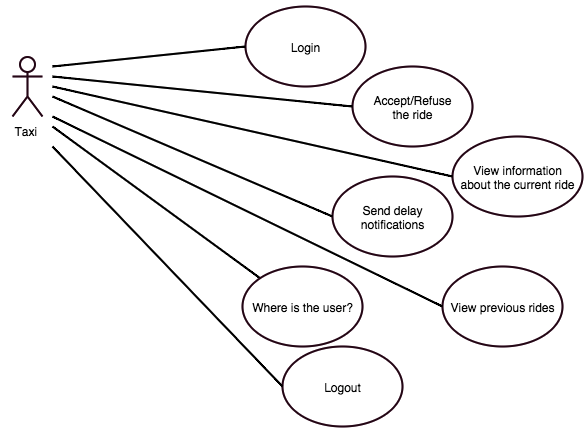
\includegraphics[width=0.70\textwidth]{./images/UseCaseTaxi.png}~
			\end{center}
		
		\subparagraph{Login}
		~\\[0.2cm]
		\vspace{20pt}
		\noindent
		\begin{tabular}{l l}
		 \textbf {Name} & Login  \\ \hline
		 \textbf{Actors} & Taxi \\ \hline
		 \textbf{Entry conditions} & No entry conditions \\ \hline
		 \textbf{Event flow} & 
		 \parbox{0.7\textwidth}{
		 \begin{enumerate}
		 \item The taxi
		    \begin{itemize}
		    \item opens the myTaxiService mobile application;
		    \item clicks on "Log in" link;
		    \item inserts username and password, after the opening of a new window;
		    \item clicks on "Confirm" link;
		    \end{itemize}
		 \item the system accepts the data inserted and the main page is shown to the taxi driver.
		 \end{enumerate}
		 } \\ \hline
		 \textbf{Exit Condition} & No exit conditions \\ \hline
		 \textbf{Exceptions} & \parbox{0.7\textwidth}{If the username and/or the password inserted don't exist in the database, an error message will be shown.}
		\end{tabular}
		
		\newpage
		\subparagraph{Confirmation/Refusal of the service}
		~\\[0.2cm]
		\vspace{20pt}
		\noindent
		\begin{tabular}{l l}
		 \textbf {Name} & Confirm/Refuse the service  \\ \hline
		 \textbf{Actors} & Taxi \\ \hline
		 \textbf{Entry conditions} & Login successful \\ \hline
		 \textbf{Event flow} & 
		 \parbox{0.7\textwidth}{
		 \begin{enumerate}
		 \item The taxi
		 \begin{itemize}
		 \item clicks on the received notification;
		 \item clicks on "Confirm" or "Refuse";
		 \end{itemize}
		 \item the system
		  \begin{itemize}
		 \item sends a notification to the user, if the taxi confirms the service;
		 \item otherwise searches the next available taxi in the queue.
		 \end{itemize}
		 \end{enumerate}
		 } \\ \hline
		 \textbf{Exit Condition} & No exit conditions \\ \hline
		 \textbf{Exceptions} & No exceptions.
		\end{tabular}
		
		\subparagraph{View information about the current ride}
		~\\[0.2cm]
		\vspace{20pt}
		\noindent
		\begin{tabular}{l l}
		 \textbf {Name} & View information about the current ride  \\ \hline
		 \textbf{Actors} & Taxi \\ \hline
		 \textbf{Entry conditions} & Login successful \\ \hline
		 \textbf{Event flow} & 
		 \parbox{0.7\textwidth}{
		 \begin{enumerate}
		 \item The taxi clicks on "View information";
		 \item the system loads from the database the information of the current ride.
		 \end{enumerate}
		 } \\ \hline
		 \textbf{Exit Condition} & No exit conditions \\ \hline
		 \textbf{Exceptions} & No exceptions.
		\end{tabular}
		
		\newpage
		\subparagraph{Send delay notifications}
		~\\[0.2cm]
		\vspace{20pt}
		\noindent
		\begin{tabular}{l l}
		 \textbf {Name} & Send delay notification  \\ \hline
		 \textbf{Actors} & Taxi \\ \hline
		 \textbf{Entry conditions} & Login successful \\ \hline
		 \textbf{Event flow} & 
		 \parbox{0.7\textwidth}{
		 \begin{enumerate}
		 \item The taxi clicks on "Send delay notification";
		 \item the system advises the user about the delay.
		 \end{enumerate}
		 } \\ \hline
		 \textbf{Exit Condition} & No exit conditions \\ \hline
		 \textbf{Exceptions} & No exceptions.
		\end{tabular}
		
		\subparagraph{View previous rides}
		~\\[0.2cm]
		\vspace{20pt}
		\noindent
		\begin{tabular}{l l}
		 \textbf {Name} & View information about the previous rides  \\ \hline
		 \textbf{Actors} & Taxi \\ \hline
		 \textbf{Entry conditions} & Login successful \\ \hline
		 \textbf{Event flow} & 
		 \parbox{0.7\textwidth}{
		 \begin{enumerate}
		 \item The taxi clicks on "View history";
		 \item the system loads from the database the information of all the previous rides.
		 \end{enumerate}
		 } \\ \hline
		 \textbf{Exit Condition} & No exit conditions \\ \hline
		 \textbf{Exceptions} & No exceptions.
		\end{tabular}
		
		\subparagraph{Where is the user?}
		~\\[0.2cm]
		\vspace{20pt}
		\noindent
		\begin{tabular}{l l}
		 \textbf {Name} & Where is the user?  \\ \hline
		 \textbf{Actors} & Taxi \\ \hline
		 \textbf{Entry conditions} & Login successful \\ \hline
		 \textbf{Event flow} & 
		 \parbox{0.7\textwidth}{
		 \begin{enumerate}
		 \item The taxi clicks on the button "Where is the user?";
		 \item the system sends an SMS to the user to tell him/her that the taxi is arrived.
		 \end{enumerate}
		 } \\ \hline
		 \textbf{Exit Condition} & No exit conditions \\ \hline
		 \textbf{Exceptions} & No exceptions.
		\end{tabular}